\chapter{Implementation}
\label{05:chapter:title}

This chapter is devoted to the implementation of additional functionality (i.e., parallelism) into the test framework within the Strimzi project.
Implementation Listings (f.e.,~\ref{interface:resourcetype},~\ref{interface:implementation:kafka}\dots) are presented in Java programming language.
Moreover, in Section~\ref{05:sec:method:wide:parallelism} we describe an implementation of the first possible level of
parallelism for more minor instances of the Kubernetes cluster.
Finally, for more comprehensive instances (i.e., multi-node Kubernetes clusters),
we explain the implementation of even higher-level parallelism in Section~\ref{05:sec:class:wide:parallelism}.

The author contributed the given code to the open-sourced project Strimzi available on
Github\footnote{Strimzi Github repository \---\ \url{https://github.com/strimzi/strimzi-kafka-operator}}.
Specifically, these changes can be found in the \emph{systemtest} module\footnote{systemtest module \---\ \url{https://github.com/strimzi/strimzi-kafka-operator/tree/main/systemtest}}.
Installation and configuration of individual parallelisation levels are described in Appendix~\ref{30:appendix:a}.
Eventually, we move more complex and extensive code snippets into Appendix~\ref{30:appendix:b}.

\section{Stage \---\ method-wide parallelisation}
\label{05:sec:method:wide:parallelism}

In this section, we describe the solutions of the individual steps proposed in Section~\ref{04:methodwideparalelisation},
which were necessary to perform for adaptation to method-wide parallelisations.
We start with an explanation of how to resolve the uniqueness of test resources in Section~\ref{05:sub:sec:unique}.
Furthermore, we describe the core implementation, and the necessary reworking of test resources, as well as \emph{ResourceManager} in Section~\ref{05:sub:sec:resourcemanager}.
Next, in Section~\ref{05:sub:sec:annotations} the author present a mechanism that determines whether a given test case has to be executed in parallel or isolation.
Finally, in Section~\ref{05:sub:sec:configuration} we explain how such parallelization can be configured,
and in Section~\ref{05:sub:sec:applicability} we describe its usability within our infrastructure.

\subsection{Unique Naming for each resource\protect\footnote{\url{https://github.com/strimzi/strimzi-kafka-operator/pull/4092}}}
\label{05:sub:sec:unique}

Several sources (f.e., \emph{Kafka cluster}, \emph{KafkaConnect}, \emph{KafkaMirrorMaker}), which are used in test cases,
are necessary to work with unique names to avoid conflict (f.e., replace existing or already created resource).
That is why we created the class \emph{TestStorage}\footnote{TestStorage \---\ https://github.com/strimzi/strimzi-kafka-operator/pull/5446/},
which will include unique generated name of the necessary resources (i.e., name of the \emph{Namespace}, \emph{Kafka cluster},
\emph{KafkaTopic}, \emph{Producer}, \emph{Consumer}).
All this is possible thanks to \emph{ExtensionContext}, where each test case has a different \emph{ExtensionContext},
and therefore it can be used as a map repository.

\subsection{Resource Manager re-work\protect\footnote{\url{https://github.com/strimzi/strimzi-kafka-operator/pull/4137}}}
\label{05:sub:sec:resourcemanager}

As described in Section~\ref{04:architecturechanges}, we created \emph{Interface ResourceType <T extends HasMetadata>}.
Where \emph{T} is a generic type and can take subtypes (f.e., Kafka, KafkaBridge, KafkaMirrorMaker).
In other words, everything that contains the object \emph{HasMetadata}\footnote{HasMetadata \---\ is an interface of
Kubernetes resources that contain metadata object}.
Listing~\ref{interface:resourcetype} shows the individual method signatures in the given interface.

\begin{lstlisting}[language=Java,label=interface:resourcetype,caption=Interface used across all resources,frame=tb]
public interface ResourceType<T extends HasMetadata> {
    String getKind();
    T get(String namespace, String name);
    void create(T resource);
    void delete(T resource);
    boolean waitForReadiness(T resource);
}
\end{lstlisting}
Each resource then signs a contract with the ResourceType interface in our test framework.
For instance, the \emph{Kafka} resource implementation (Listing~\ref{interface:implementation:kafka}).
\begin{lstlisting}[language=Java,label=interface:implementation:kafka,caption=Kafka resource sings contract with ResourceType interface,frame=tb]
public class KafkaResource implements ResourceType<Kafka> {
    @Override
    public String getKind() {  return Kafka.RESOURCE_KIND;}
    @Override
    public Kafka get(String namespace, String name) {...}
    @Override
    public void create(Kafka resource) {...}
    @Override
    public void delete(Kafka resource) {...}
    @Override
    public boolean waitForReadiness(Kafka resource) {...}
    // implementation of each methods omitted for clarity
}
\end{lstlisting}

Nevertheless, the most critical part of the entire Strimzi test framework is \emph{ResourceManager}.
As described in the design~\ref{04:sub:sec:resourcemanager}, so instead of three stacks (i.e., pointer, class and method),
we had to adapt a solution with hash maps, which for each test case will keep each stack in which will contain the test resources.
At the same time, thanks to the proposed algorithms (\ref{04:alg:creationofresource},~\ref{04:alg:deleteresources}),
the algorithm for creating resources according to the generic type \emph{T}, finds out which method to invoke.
Moreover, a parallel algorithm for deleting individual resources from a given stack.
Finally, the~\ref{04:alg:syncresources} algorithm for synchronization of parallel generating resources is most useful
in the parallel preparation of individual resources for a given test case.
An example of such a preparation phase (Listing~\ref{resourcemanager:sync:method}).
\begin{lstlisting}[language=Java,label=resourcemanager:sync:method,caption=Example of parallel preparation of resources,frame=tb]
// create resources in parallel (simultaneously)
resourceManager.createResource(extensionContext, false,
    KafkaTemplates.kafka().build()
    KafkaTemplates.kafkaWithMetrics().build(),
    KafkaMirrorMakerTemplates.kafkaMirrorMaker().build(),
    KafkaConnectTemplates.kafkaConnect().build(),
    KafkaClientsTemplates.kafkaClients().build()
);
// synchronize point (barrier)
resourceManager.synchronizeResources(extensionContext);
\end{lstlisting}
The overall implementation of individual algorithms (\ref{04:alg:creationofresource},~\ref{04:alg:syncresources} and~\ref{04:alg:deleteresources})
can be seen in the Appendix~\ref{30:appendix:b}.

\subsection{Injection of the runtime annotations}
\label{05:sub:sec:annotations}

Another crucial part is creating a mechanism that will provide information, which test case may be executed in parallel
mode or run in complete isolation.
In Section~\ref{04:methodwideparalelisation}, we propose such annotations offered by the Java language.
We implemented three types of annotations for method-wide parallelisation.
The most concise annotation is \emph{@ParallelTest}, which overrides the parallelism configuration at runtime.
It is possible to see the given implementation of such an annotation on Listing~\ref{annotation:paralleltest}.
An essential part is \emph {@Execution(ExecutionMode.CONCURRENT)}, where the semantics of this line means that the given
annotation will overwrite the given configuration from a sequential mode to parallel mode and thanks to \emph {@Retention(RUNTIME)} it will do so at runtime.

\begin{lstlisting}[language=Java,label=annotation:paralleltest,caption=Implementation of the @ParallelTest annotation,frame=tb]
@Target(ElementType.METHOD)
@Retention(RUNTIME)
@Execution(ExecutionMode.CONCURRENT)
@ResourceLock(mode = ResourceAccessMode.READ, value = "global")
@Test
public @interface ParallelTest {  }
\end{lstlisting}
Another annotation (Listing~\ref{annotation:isolatedtest}) we have implemented to be responsible for the complete isolation of is \emph{@IsolatedTest}.
At an initial glance, it is remarkably similar to the previous annotations.
However, there is one major difference when using \emph{@ResourceLock}.
When \emph {@ParallelTest} uses a read lock, \emph{@IsolatedTest} uses a \emph{read\_write} lock.
The idea is that \emph{read\_write} lock will completely isolate us from other tests.
Multiple \emph{@ParallelTest} will be performed at the same time, and \emph{@IsolatedTest} will wait until this lock is
released (because these two annotations share the same @ResourceLock named \emph{global}).

\begin{lstlisting}[language=Java,label=annotation:isolatedtest,caption=Implementation of the @IsolatedTest annotation,frame=tb]
@Target(ElementType.METHOD)
@Retention(RUNTIME)
@Inherited
@ResourceLock(mode = ResourceAccessMode.READ_WRITE, value = "global")
@Test
public @interface IsolatedTest {
    String value() default ""; // reason why it needs isolation
}
\end{lstlisting}
Eventually, we implemented the last annotation due to product requirements \emph{@ParallelNamespaceTest}.
This annotation is equivalent to \emph{@ParallelTest}, but there is a slight distinction.
We create an additional namespace for each test case.
Scenarios where we mainly used it is when multiple Kafka clusters are deployed for a given test or when we use
\emph{KafkaMirrorMaker} (by default, we need two Kafka clusters).

\subsection{Configuration}
\label{05:sub:sec:configuration}

The method-wide parallelization configuration can be set up in several ways (a) using system properties (Listing~\ref{config:system:property}),
(b) using the junit-platform.properties configuration file (Listing~\ref{config:file}).
\begin{lstlisting}[language= Java,label=config:system:property,caption=(a) Configuration via system properties,frame=tb]
-Djunit.jupiter.execution.parallel.enabled = true
-Djunit.jupiter.execution.parallel.config.fixed.parallelism = <n>
// parallel.mode.default has default value same_thread
// parallel.mode.classes.default has default value same_thread
\end{lstlisting}
In both cases, \emph{n} threads will be released, where each thread will perform one test case at a time, and if it finishes its work,
it will move on to the next test case. This is repeated until there is no more test to execute in the given test class.
\begin{lstlisting}[language=Java,label=config:file,caption=(b) Configuration via file,frame = tb]
junit.jupiter.execution.parallel.enabled = true
junit.jupiter.execution.parallel.mode.default = same_thread
junit.jupiter.execution.parallel.mode.classes.default = same_thread
junit.jupiter.execution.parallel.config.strategy = fixed
junit.jupiter.execution.parallel.config.fixed.parallelism = <n>
\end{lstlisting}

\subsection{Applicability}
\label{05:sub:sec:applicability}

Method-wide parallelization for our testing framework is most efficient for more diminutive infrastructures,
typically with parameters f.e., 24GB RAM and eight cores. We use such infrastructure as part of nightly testing.
In the circumstances, we have less power available; it is necessary to count on it that in more demanding test cases
(i.e., a test case using \emph{KafkaMirrorMaker} or several Kafka clusters), the cluster will be unstable, which will
lead to poor test results and overall test timeouts. On the other hand, in the case of more powerful infrastructure
(i.e., multi-node Kubernetes cluster), it is possible to use the following form of parallelism.

\section{Stage \---\ class-wide parallelisation}
\label{05:sec:class:wide:parallelism}

In this section, we explain the solutions of the individual steps proposed in Section~\ref{04:classwideparalelisation},
which were necessary to perform for adaptation to class-wide parallelisations.
We first describe complete re-work of Cluster Operator installation in Section~\ref{05:class:wide:shared:co}.
Next, in Section~\ref{05:sub:sec:isolation:of:test:suites} and Section~\ref{05:class:wide:suite:thread:controller}
the author exemplify mechanism for isolation of test suites and describe common problems in relation of isolation.
Moreover, we present another component required for class-wide parallelisation
and management of all \emph{Namespaces} in Section~\ref{05:class:wide:test:namespace:manager}.
Finally, in Section~\ref{05:class:wide:config} we explain how such parallelisation can be configured, and
in Section~\ref{05:class:wide:application} we describe its usability within our infrastructure.

\subsection{Deployment of shared Cluster Operator across $\forall$ suites}
\label{05:class:wide:shared:co}

As we proposed in Section~\ref{05:sharedclusteroperator} for class-wide parallelisation,
we want to create a shared Cluster Operator alongside all test classes.
Such an approach is possible thanks to root \emph{ExtensionContext}, which guarantees that the Cluster Operator instance
will be deleted only after the overall execution. We will describe the two primary phases of our proposed JUnit5 extension
(i.e., \emph{BeforeAllOnce} setup phase - Listing~\ref{before:all:once}).
The method must use synchronized to prevent multiple threads in a race condition.
This situation would occur if two or more \emph{@ParallelSuite} threads passed the \emph{!BeforeAllOnce.systemReady}
condition and then started to create a two times instance of the Cluster Operator.
At the same time, we may notice that it is necessary to change the configuration of the given Cluster Operator for different configurations.

\begin{lstlisting}[language= Java,label=before:all:once,caption=Setup phase of shared Cluster Operator,frame=tb]
synchronized private static void systemSetup(
    ExtensionContext extensionContext) {
    if (!BeforeAllOnce.systemReady) {
        sharedExtensionContext = extensionContext.getRoot();
        if (StUtils.isParallelSuite(extensionContext)) {
            BeforeAllOnce.systemReady = true;

            if (Environment.isNamespaceRbacScope() &&
                !Environment.isHelmInstall()) {
            clusterOperator = new SetupClusterOperator
                .SetupClusterOperatorBuilder()
                .withExtensionContext(sharedExtensionContext)
                .createInstallation()
                .runInstallation();
            } else {
            // setup cluster operator before all suites only once
                clusterOperator = new SetupClusterOperator
                .SetupClusterOperatorBuilder()
                .withExtensionContext(sharedExtensionContext)
                .withNamespace(Constants.INFRA_NAMESPACE)
                .withWatchingNamespaces(Constants.WATCH_ALL_NAMESPACES)
                .createInstallation()
                .runInstallation();
            }
        }
        sharedExtensionContext.getStore(ExtensionContext.Namespace.GLOBAL)
            .put(SYSTEM_RESOURCES, new BeforeAllOnce());
    }
}
\end{lstlisting}
The last essential aspect is the last line in Listing~\ref{before:all:once}, where we create an instance of the given
extension and thus implicitly call the \emph{close()} method.
The class implements the \emph{Autocloseable} Interface, which ensures that such a method is called at the end of an instance's life.
Inside the \emph{close()} method, we have to reset the flag counter and also call the
\emph{Singleton}\footnote{Singleton pattern \---\ it is one of the creational design patterns, restricting instantiation of the class to only one instance.
Thus invocation of the \emph{getInstanceHolder} method results always in the same instance.} instance of the shared Cluster Operator
to uninstall all components (Listing \ref{before:all:once:teardown}).


\begin{lstlisting}[language= Java,label=before:all:once:teardown,caption=Teardown phase of shared Cluster Operator,frame=tb]
public synchronized void close() throws Exception {
    BeforeAllOnce.systemReady = false;
    // complete un-install all components
    SetupClusterOperator.getInstanceHolder().unInstall();
}
\end{lstlisting}

Furthermore, recall from Section~\ref{05:sharedclusteroperator}, when we proposed the unification of the Cluster Operator configuration
option via the Builder design pattern.
Due to the numerous factory methods already becoming difficult to manage, it was necessary.
The overall implementation without auxiliary methods (omitted for brevity) can be found in Listing~\ref{cluster:operator:builder:pattern}.

The last part we proposed in Section~\ref{05:sharedclusteroperator} was the \emph{Rollback} algorithm (\ref{05:alg:rollback}).
This is necessary if we have a situation of two classes that require a distinct configuration of the Cluster Operator f.e.,
Thread A terminates the execution of test class \emph{X} and thread B will start execution of test class \emph{Y},
which needs a default configuration\footnote{Default configuration \---\ Such configuration is used alongside with \emph{@ParallelSuite}.
Thus if @IsolatedSuite ends its execution and starts @ParallelSuite, it always comes with triggering \emph{Rollback} algorithm.} that differs from the current.
In such a situation, we trigger the \emph {Rollback} algorithm.

\subsection{Isolation of test Suites}
\label{05:sub:sec:isolation:of:test:suites}

The problem of isolating several classes that need different Cluster Operator configurations has been described and explained in Section~\ref{05:isolatedsuite}.
So we implemented an annotation, which primarily serves as a label for that class.
\begin{lstlisting}[language=Java,label=annotation:isolatedsuite,caption=Implementation of the @IsolatedSuite annotation,frame=tb]
@Retention(RetentionPolicy.RUNTIME)
@Target({ElementType.TYPE })
public @interface IsolatedSuite {  }
\end{lstlisting}
Moreover, we have implemented an additional mechanism that will ensure synchronisation between such test suites
(i.e., \emph{@IsolatedSuite}. We create \emph{SuiteThreadController} class, and one of the synchronisations that are
implemented inside this class is for \emph {@IsolatedSuite}. If \emph{@IsolatedSuite} starts its execution, it sets the given
boolean value to true, which prevents the following thread from going through the given while loop.
If \emph{@IsolatedSuite} completes its execution, it sets the given boolean value to false, and
the following thread will be able to start its execution. Furthermore, we notice the keyword \emph{synchronised}
in the method definition. The main reason why this keyword is necessary is that for multiple threads (i.e., \emph{@IsolatedSuite}),
they will have to wait until the thread that is currently in the loop is dropped and unlocks the lock, which implicitly
adds \emph {synchronised} (Listing~\ref{isolatedsuite:sync}).

\begin{lstlisting}[language=Java,label=isolatedsuite:sync,caption=Implementation of the @IsolatedSuite synchronisation mechanism,frame=tb]
public synchronized void waitUntilEntryIsOpen(
    ExtensionContext extensionContext) {
    // only one thread at a time
    while (this.isOpen.get()) {
        // Suite Y is waiting to lock to be released.
        Thread.currentThread().sleep(...);
    }
    // Suite X has locked the @IsolatedSuite and other
    // @IsolatedSuites must wait until lock is released.
    this.isOpen.set(true);
}
\end{lstlisting}

\subsection{SuiteThreadController}
\label{05:class:wide:suite:thread:controller}

As mentioned in Section~\ref{05:sub:sec:isolation:of:test:suites}, the \emph{SuiteThreadController} class provides multiple synchronizations.
We have already described the first type in the previous Section for \emph{@IsolatedSuite} classes.
However, there are several other scenarios between classes (i.e., @ParallelSuite and @IsolatedSuite) that can occur:
\begin{enumerate}[itemsep=1mm, parsep=0pt]
    \item case \---\ only \emph{@ParallelSuite} will be executed, (no need synchronisation)
    \item case \---\ only \emph{@IsolatedSuite} will be executed, (Section~\ref{05:sub:sec:isolation:of:test:suites})
    \item case \---\ several \emph{@ParallelSuite} will be executed followed by a few \emph{@IsolatedSuite},
    \item case \---\ several \emph{@IsolatedSuite} will be executed followed by a couple of \emph{@ParallelSuite},
    \item case \---\ \emph{@ParallelSuite} starts, then \emph{@IsolatedSuite} and finally \emph{@ParallelSuite},
    \item case \---\ \emph{@IsolatedSuite} starts, then \emph{@ParallelSuite} and finally \emph{@ParallelSuite}.
    \item case \---\ ForkJoinPool spawning additional threads, which exceeding our configured parallelism limit.
\end{enumerate}
In the first case, it is clear that we will not need any synchronisation between classes because they all use the same
Cluster Operator configuration. Nevertheless, in the third case, it is necessary to provide some form of synchronisation.
The scenario that could occur is that @IsolatedSuite would be the last to be executed, and at the same time, our testing
framework runs a few @ParallelSuite. However, this means nothing for @IsolatedSuite, because no lock is attached to it,
and it would start modifying the shared Cluster Operator and thus disrupt the execution of @ParallelSuite classes.
Therefore, we have implemented an atomic counter into the \emph{SuiteThreadController} class, which will increase
if the thread starts executing @ParallelSuite and decreases it as soon as it completes. Subsequently, the thread
(i.e., @IsolatedSuite) that wants to start executing will not be able to start until the @ParallelSuite counter is equal to zero.
In this case, the previous possible pessimistic scenario is eliminated (Listing~\ref{parallelsuite:isolatedsuite:sync}).

\begin{lstlisting}[language=Java,label=parallelsuite:isolatedsuite:sync,caption=@ParallelSuite and @IsolatedSuite synchronisation mechanism,frame=tb]
public void waitUntilZeroParallelSuites(
    ExtensionContext extensionContext) {
    // until more that 0 parallel suites running in parallel 'active waiting'
    boolean preCondition = true;

    while (preCondition) {
        Thread.sleep(...);

        // runningTestSuitesInParallelCount variable is
        // changed by other threads (i.e., @ParalleSuites)
        preCondition = runningTestSuitesInParallelCount.get() > 0;
    }
}
\end{lstlisting}

For the fourth case, when we start executing a few @IsolatedSuite and then @ParallelSuite, we can reduce this to the
problem when we only run the @IsolatedSuite (2nd case) because it is necessary to synchronise between @IsolatedSuite
and none for @ParallelSuite.

In the fifth case, when we begin to execute @ParallelSuite, then several @IsolatedSuite, we eventually start running several
@ParallelSuite. Thus, this includes the combination of synchronisation from cases 2 and 3.
The analogy for the sixth case is a combination of these two cases.

The last case synchronisation is required when ForkJoinPool spawns multiple threads that exceed our configured parallelism limit.
It does this because ForkJoinPool uses a worker-steal algorithm. Unfortunately, this technique spawns additional threads when
synchronisation primitive blocks thread (f.e., this can lead to a situation where the user sets a fixed value of parallelism
to two when he expects to run at most two test classes with two test cases. However, in some borderline situations,
it could be that ForkJoinPool will spawn five threads instead of two. Because of this, we have implemented an additional
mechanism that will make such threads sleep if they exceed the value of parallelism (Listing~\ref{parallel:suite:sync}).
Noteworthy is that if @ParallelSuite completes its execution, then in @AfterAll (i.e., at the end of the test class),
it notifies and set the value of \emph{isParallelSuiteReleased} to true. Thus allow one of the waiting @ParallelSuite to start its execution.

\begin{lstlisting}[language=Java,label=parallel:suite:sync,caption=Additional synchronization for multiple @ParallelSuite\, that exceed our configured parallelism limit and are spawned by ForkJoinPool,frame=tb]
public void waitUntilAllowedNumberTestSuitesInParallel(
    ExtensionContext extensionContext) {
    final String testSuiteToWait =
        extensionContext.getRequiredTestClass().getSimpleName();
    waitingTestSuites.add(testSuiteToWait);

    // wait zone for threads, which exceed maximum
    // of allowed test suites in parallel
    while (!isRunningAllowedNumberTestSuitesInParallel()) {
        // waiting to proceed with execution but current thread
        // exceed maximum of allowed test suites in parallel
        Thread.currentThread().sleep(...);

        // release and lock again
        if (isParallelSuiteReleased.get()) {
            // lock
            isParallelSuiteReleased.set(false);
            // remove selected test suite to continue its execution
            waitingTestSuites.remove(testSuiteToWait);
            break;
        }
    }
    // selected test suite is released
}
\end{lstlisting}

\subsection{TestNamespaceManager}
\label{05:class:wide:test:namespace:manager}

Another component that is required for class-wide parallelisation is TestNamespaceManager.
Recall the @ParallelNamespaceTest annotation, creating its namespace for such a test case.
Also, assume the situation of multiple test classes (i.e., @ParallelSuites) running in parallel.
If we run more than one such class, it is necessary to ensure each test class operates with its namespace.
Of course, we can think of several approaches to solve this problem by using static information to define separate Namespaces
for each test suite that would need it. However, it would require a manual approach when we add another such test class.
Another approach, using dynamic information, would be to find out at runtime which classes will need such a namespace.
We obtain this information using the recursive method we implemented, which obtains all @ParallelSuite (Listing \ref{test:namespace:manager:list:files}).

\begin{lstlisting}[language=Java,label=test:namespace:manager:list:files,caption=Dynamically list all @ParallelSuites,frame=tb]
private void retrieveAllSystemTestsNames(File stFiles) {
    if (stFiles.getName().endsWith(Constants.ST + ".java") &&
        !stFiles.getName().contains(Constants.ISOLATED)) {
        this.stParallelSuitesNames.add(stFiles.getName());
    }
    File[] children = stFiles.listFiles();
    if (children == null) {
        return;
    }
    for (File child : children) {
        retrieveAllSystemTestsNames(child);
    }
}
\end{lstlisting}
Subsequently, we will make a namespace for each of these classes and store it in a hash map where the key will be the class name
(f.e., \emph{TracingST.getClass().getName()}), and if the given test class wants to get this namespace it will do so simply as
illustrated in Listing \ref{test:namespace:manager:get:namespace}.

\begin{lstlisting}[language=Java,label=test:namespace:manager:get:namespace,caption=@ParallelSuite query generated (dynamically) namespace,frame=tb]
@ParallelSuite
class TracingST {
    private final String namespace =
        testSuiteNamespaceManager.getMapOfAdditionalNamespaces()
            .get(TracingST.class.getSimpleName())
            .stream()
            .findFirst()
            .get();
    // other attributes ommited for brevity...
}
\end{lstlisting}

\subsection{Configuration}
\label{05:class:wide:config}

Recall from Section~\ref{05:sub:sec:configuration}, where we present configuration of the method-wide parallelisation.
To enable class-wide parallelisation, we can use two ways same as describe in Section~\ref{05:sub:sec:configuration} but
with different values (a) using system properties (Listing~\ref{config:system:property}),
(b) using the junit-platform.properties configuration file (Listing~\ref{config:file}).
Note that we have to override system property parallel.mode.classes.default to concurrent.
With that we can run multiple test classes simultaneously.
Moreover, we may notice that the system property parallel.mode.default is not concurrent.
That is because we override this value using the annotations @ParallelTest and @ParallelNamespaceTest.
\begin{lstlisting}[language= Java,label=config:system:property,caption=(a) Configuration via system properties,frame=tb]
-Djunit.jupiter.execution.parallel.enabled = true
-Djunit.jupiter.execution.parallel.mode.classes.default= concurrent
-Djunit.jupiter.execution.parallel.config.fixed.parallelism = <n>
\end{lstlisting}
\begin{lstlisting}[language=Java,label=config:file,caption=(b) Configuration via file,frame = tb]
junit.jupiter.execution.parallel.enabled = true
junit.jupiter.execution.parallel.mode.default = same_thread
junit.jupiter.execution.parallel.mode.classes.default = concurrent
junit.jupiter.execution.parallel.config.strategy = fixed
junit.jupiter.execution.parallel.config.fixed.parallelism = <n>
\end{lstlisting}

\subsection{Applicability}
\label{05:class:wide:application}

The class-wide parallelism for our testing framework is used mainly in the more extensive infrastructures we have at our disposal
(i.e., multi-node Kubernetes or Openshift cluster, where each node has 8 CPU cores and 16GB RAM).
Therefore, the implemented solution was tested on AWS infrastructures and, at the same time Openstack.
The question is, what is the optimal configuration for each infrastructure (Listing~\ref{07:fig:optimal:configuration:infrastructure}).
The next chapter, which is devoted to experimentation, can answer such a question.

\begin{figure}[!ht]
\centering
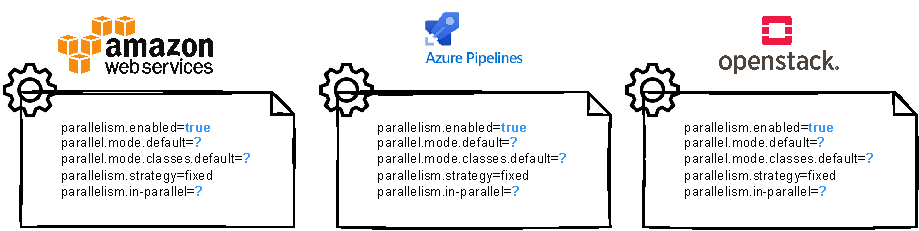
\includegraphics[scale=0.9]{obrazky-figures/07-implementation/01-configuration}
\caption{Find optimal configuration for each infrastructure}
\label{07:fig:optimal:configuration:infrastructure}
\end{figure}

\section{Complications during implementation (Do we need it??)}

\chapter{Experimental evaluation}
\label{06:chapter:title}

\section{Experimental setup}
%\subsection{Azure \& Openstack clouds (podkapitola nebude vidieť...)}
\section{Results}
\section{Evaluation of the obtained results}

\chapter{Future work}
\label{07:chapter:title}


\chapter{Conclusion}
\label{08:chapter:title}
